\subsection[Studiengebühren]{Studiengebühren --\\ eine abschließende
Betrachtung}
\emph{von Henning Günther}

Wir schreiben das Wintersemester 2009/10.
Der Widerstand gegen Studiengebühren liegt in Trümmern.
Nach den vernichtenden Niederlagen im voll\-stän\-di\-gen Boykott der
Studiengebühren im Sommersemster 2007, an dem nur 504 der über 14.000 Studenten teilnahmen und dem darauf folgenden, kaum noch spürbaren ,,5 Euro''-Boykott im Wintersemester 2007/08 sind die Studenten kaum noch zu Widerstand bereit. Im Sommersemster 2008 war das Werk vollbracht, jeder anfängliche Widerstand in alle Winde zerstreut, die anfänglich so breit erscheinende Front der Studiengebührengegner zerschlagen.

Was war geschehen?
Wie konnte sich die vormals so rebellische Studentenschaft, die früher keine Möglichkeit ausließ, gegen das Unrecht zu protestieren, innerhalb von nur einem Jahr in einen in gedemütigter Haltung die Gebühren entrichtenden Haufen Elend verwandeln?

Es hat den Anschein, dass die diabolisch geniale Saat der
Studiengebühren-Fürsprecher, die Daumenschrauben der ,,Campus-Maut'' nicht
sofort und im vollen Umfang anzuziehen, auf ganzer Linie aufgegangen sei. Denn es traf zunächst die, die sich am wenigsten wehren konnten: An Erstsemestern die, da noch nicht eingeschrieben, keinen Boykott wagen
konnten wurde zuerst erprobt, ob 500 Euro ein Preis waren, für den die Studenten zu kämpfen bereit wären. Sie waren es nicht.
Zwar waren viele ,,im Prinzip'' dagegen, taten diese Meinung aber nur mäßig
auf den wenigen Demonstrationen kund.

Die meisten der Studenten scheinen sich inzwischen mit dem Fakt, mit jährlich
1000 Euro weniger auskommen zu müssen, abgefunden zu haben. Kaum jemand gibt sich noch dem Wunschtraum hin, größere Teile der Studenten für irgendeine Form des organisierten Protest zu begeistern.
Es scheint fast als könnten die Studiengebührenschergen bald wieder Morgenluft wittern und in der Lage sein, dank mangelnden Widerstand, ihre kühnsten Träume zu verwirklichen: 1000 Euro Studiengebühren pro Semester und mehr.

Was wird die Zukunft bringen?
Werden die Besiegten weiterhin wie die Gespenster einer längst vergangenen Zeit durch die Unigänge huschen, von einer Vorlesung zur nächsten hetzen, um sich durch ein schnelleres Studium vielleicht ein paar Euro Studiengebühren zu sparen und gelernt haben, stets mit der Angst vor einer Erhöhung der Gebühren zu leben?
Es bleibt zu hoffen dass den Advokaten des Bezahlstudiums dieser Triumph nicht gewährt wird.
%
\end{multicols}
\begin{center}
  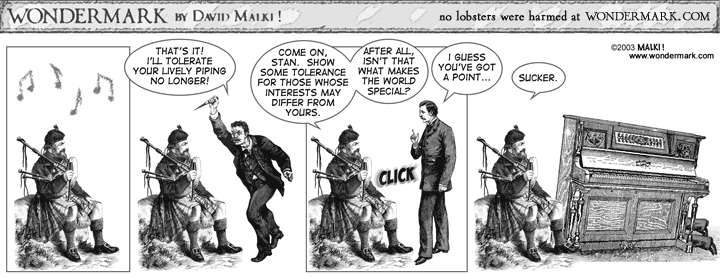
\includegraphics[width=\linewidth]{bilder/comics/wondermark003.png}
\end{center}
%
%
\begin{multicols}{2}
